\documentclass[10pt]{article}

\usepackage{fullpage}
\usepackage[margin=2cm]{geometry}
\usepackage[pdftex]{graphicx}
\usepackage{float}

\begin{document}

\title{\vspace{-2cm}ARM11 Final Report}
\author{\small Alexander CLARKE, Qiang FENG, Jordan SPOONER, Laurence SQUIRES}

\maketitle

\section{ARM11 Emulator and Assembler}

The folder structure for the project is as follows:

\begin{itemize}
\item \texttt{src/} holds the \texttt{emulate.c} and \texttt{assemble.c} files, as well as files used by both emulate and assemble.
\item \texttt{src/emulate\_utils/} contains the files containing the constants, structs and helper functions used by emulate.
\item \texttt{src/assemble\_utils/} contains the files containing the constants, structs and helper functions used by assemble.
\end{itemize}

\subsection{Emulator Implementation}

See \texttt{doc/Checkpoint.pdf} for a brief overview of our implementation and \texttt{doc/LaTeX Documentation/refman.pdf} for full documentation.

\begin{figure}[H]
\begin{minipage}{0.5\linewidth}

\subsection{Assembler Implementation}

We structured our assembler as follows:

\begin{itemize}
\item \texttt{assemble.c} contains the function \texttt{main}, which takes two arguments. The first is a filename for a text file containing valid ARM11 assembly instructions. The second is a filename to which the assembled ARM11 binary object code is written. \texttt{main} is responsible for reading in the assembly instructions, tokenizing them using the helper functions in \texttt{tokenize.c}, creating a symbol table, assembling the tokenized input using the helper functions in \texttt{assembler.c}, and writing the object code to a binary file. It is also responsible for freeing any remaining allocated memory in order to avoid memory leaks.
\item \texttt{unit\_tests.c} contains a simple test suite that uses assertions to check that called functions meet their documented functionality.
\end{itemize}

\end{minipage}
\hspace{0.05\linewidth}
\begin{minipage}{0.45\linewidth}

\centering
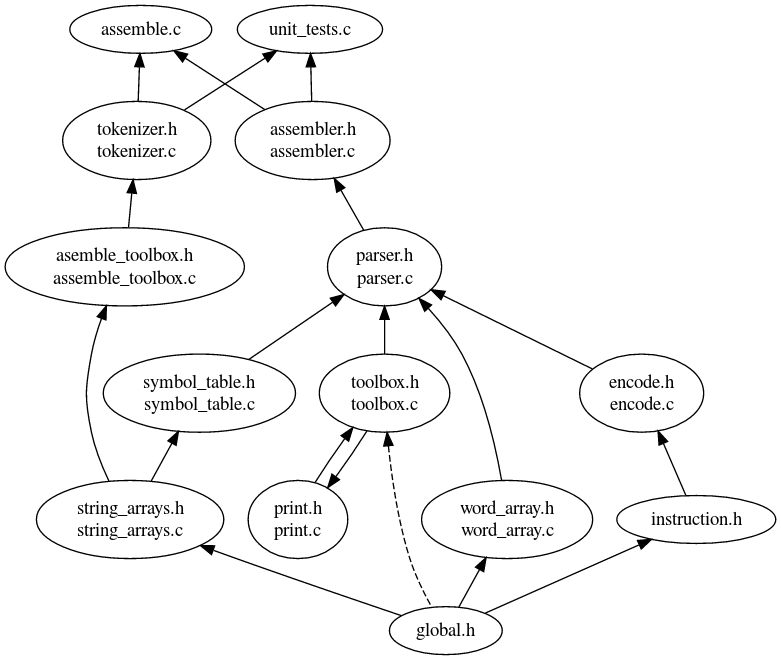
\includegraphics[scale=0.28]{Report/assemble.png}
\caption{Dependency Graph for \texttt{assemble.c}}

\end{minipage}
\end{figure}

\begin{itemize}
\item \texttt{tokenizer.c} TODO.
\item \texttt{assemble\_toolbox.c} TODO.
\item \texttt{string\_arrays.c} TODO. \texttt{string\_array.h} TODO.
\item \texttt{assembler.c} TODO.
\item \texttt{parser.c} TODO.
\item \texttt{encode.c} TODO. \texttt{instruction.h} TODO.
\item \texttt{symbol\_table.c} TODO.
\item \texttt{word\_array.c} TODO.
\item \texttt{toolbox.c} TODO.
\item \texttt{global.h} TODO.
\end{itemize}

See \texttt{doc/LaTeX Documentation/refman.pdf} for full documentation.

\subsection{Quality Assurance and Testing}

\subsubsection{Quality Assurance}

\paragraph{Style Guide}
TODO.

\paragraph{Code Reviews}
TODO.

\subsubsection{Testing}

\paragraph{Automated Testing}
TODO.

\paragraph{Unit Tests}
TODO.

\paragraph{Memory Checks}
TODO.

\paragraph{Ruby Test Suite}
TODO.

\section{Terminal-based Motion-controlled Game Engine using OpenCV}

\subsection{Introduction}

Our group’s chosen extension comes in two parts. The first part is a versatile ASCII-graphics game engine. The second part is a hand tracking program built using OpenCV. Together they can be used to create simplified kinetic type game system. The game engine can be used to create many different 2D games. We created both flappy bird and snake to show its utility. The games can be controlled by keyboard or using our hand tracking program. Our hand tracking program uses a webcam to return the position of where it believes the hands are which would then be used by our game engine. Together they create an engaging game experience.

\subsection{Implementation}

\subsubsection{Terminal-based ASCII Game Engine}

TODO. Discussion of difficulties.

\subsubsection{Hand Tracking using OpenCV}

TODO. Discussion of difficulties.

\subsection{Quality Assurance and Testing}

TODO.

\section{Project Evaluation}

\subsection{Group Working and Communication}

Our group initially came together to work out what structure our project would have. We then worked out all of the data types that we would need to implement our design for the structure and then implemented them. Using these, we came up with function prototypes.

Our group created a shared Google Docs spreadsheet to track all of the functions we thought we needed to implement. There were three jobs for each function. These were: complete the code, create unit tests for the code and review (and sign off) the code. We then assigned jobs to different team members, but sometimes we completed other people's jobs if it improved our groups workflow. Often we would implement functions inside different files to make version control easier.

We found that the most effective form of communication was always face-to-face, so we tried to spend as much time as possible in the Computing labs, where communication was easiest. At other times, we were able to continue working by using Slack and our shared spreadsheet.

Overall, our group worked well together. The communication and organisation between members in our group meant that we were always aware of what we should be doing, and also what other members were doing. We split up the work well, with all members of the team contributing fairly equally.

\paragraph{Benefits}
TODO.

\paragraph{Drawbacks}
TODO.

\subsection{Individual Reflections}

\paragraph{Alexander CLARKE}
TODO.

\paragraph{Qiang FENG}
TODO.

\paragraph{Jordan SPOONER}
TODO.

\paragraph{Laurence SQUIRES}
TODO.

\end{document}
